\chapter{Imagens}

As imagens são uma parte importante no design de uma página web. Elas podem ajudar a transmitir uma mensagem, destacar informações importantes e tornar uma página mais atraente visualmente. Além disso, as imagens também podem ser usadas para fornecer informações adicionais, como diagramas, gráficos e ilustrações.

No entanto, incluir imagens em uma página web é mais do que simplesmente fazer upload delas e inseri-las no código. É importante ter em mente questões como o formato de imagem, a otimização para a web e a responsividade.

Neste capítulo, vamos explorar as melhores práticas para incluir imagens em páginas web, incluindo como adicionar imagens a uma página HTML, escolher o formato de imagem correto e garantir que as imagens sejam exibidas corretamente em diferentes tamanhos de tela. Vamos também discutir como usar figuras, legendas e mapas de imagem, visando tornar as imagens mais significativas e esteticamente agradáveis.

\section{Adicionando Imagens a Uma Página HTML}

O elemento \var{<img>} é usado para adicionar imagens a uma página HTML. É importante observar que o elemento \var{<img>} não possui \textit{tag} de fechamento, ou seja, não tem conteúdo. Em vez disso, ele termina no final da \textit{tag} de abertura. O código \ref{code:img} mostra um exemplo de como adicionar uma imagem a uma página HTML usando o elemento \var{<img>}.

\begin{htmlcode}{Adicionando uma imagem ao documento}{code:img}
<h1>Sala de Aula</h1>
<img src="imagem1.jpg" alt="Sala de aula com alunos usando computadores.">
\end{htmlcode}

A primeira linha do exemplo de código \ref{code:img} apresenta um título. Na segunda linha, temos o elemento \var{<img>}, cujo atributo \var{src} especifica o caminho para a imagem e o atributo \var{alt} fornece uma descrição da imagem para usuários com deficiência visual ou para navegadores que não conseguem exibir a imagem. É importante incluir uma descrição precisa e informativa para o atributo \var{alt}, pois isso ajuda a garantir que o conteúdo da página seja acessível para todos. A figura \ref{fig:img} mostra o código \ref{code:img} renderizado.

\begin{figure}[ht!]    
    \frame{
    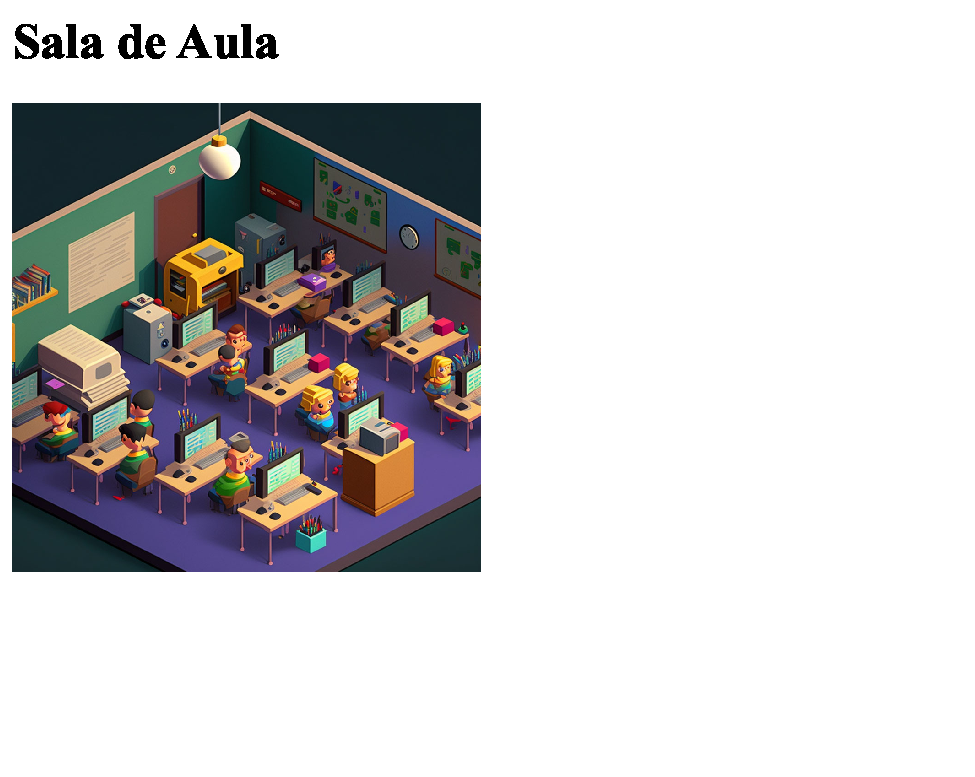
\includegraphics[width=1\textwidth, trim={0 3.25cm 0cm 0}]{Images/chapter05/imagem01.pdf}}
    \caption{Renderização da imagem do exemplo \ref{code:img}.}
    \label{fig:img}
\end{figure}

Além do \var{src} e do \var{alt}, existem outros atributos que podem ser usados com o elemento \var{<img>}. Por exemplo, o atributo \var{width} e o atributo \var{height} podem ser usados para especificar a largura e a altura da imagem, respectivamente. Vale ressaltar que, ao passar valores para ambos os atributos, devemos nos atentar para usar valores que mantenham as proporções da imagem. Caso contrário, a imagem ficará distorcida. Se você alterar o valor de um dos atributos apenas, o outro se ajusta automaticamente para manter a proporção. O código \ref{code:img2} mostra um exemplo de como adicionar uma imagem a uma página HTML usando o elemento \var{<img>} com uma largura predefinida. Neste caso, a algura será ajustada automaticamente para manter a proporção.

\begin{htmlcode}{Imagem com atributo de largura.}{code:img2}
<h1>Aluno Usando Computador</h1>
<img src="imagem2.png" alt="Aluno pensativo em frente ao computador." width="200">
\end{htmlcode}

No exemplo \ref{code:img2}, a largura da imagem é especificada como 200 pixels. Em síntese, o elemento \var{<img>} é uma ferramenta poderosa para adicionar imagens a uma página HTML. É importante lembrar de incluir descrições precisas e informativas nas imagens, além de usar outros atributos, como \var{width} e \var{height}, para controlar o tamanho da imagem. A figura \ref{fig:img2} mostra o código \ref{code:img2} renderizado.

\begin{figure}[ht!]    
    \frame{
    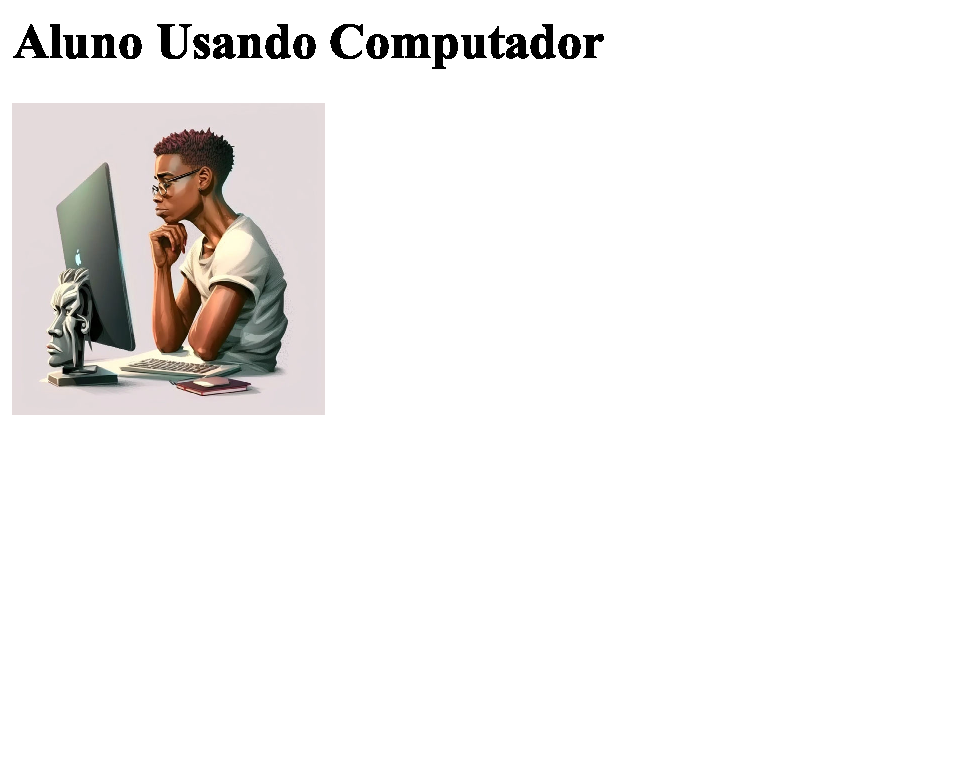
\includegraphics[width=1\textwidth, trim={0 5.9cm 0cm 0}]{Images/chapter05/imagem02.pdf}}
    \caption{Renderização da imagem do exemplo \ref{code:img2}.}
    \label{fig:img2}
\end{figure}

\section{Formatos de Imagem}

Quando se trata de incluir imagens em uma página web, é importante escolher o formato de imagem correto para garantir a qualidade da imagem, o tempo de carregamento rápido da página e a compatibilidade com diferentes navegadores.

Existem muitos formatos de imagem disponíveis, mas alguns são mais comuns na web do que outros. Nesta seção, vamos explorar os formatos de imagem mais usados na web, a saber, PNG, JPEG, GIF e SVG. Vamos discutir suas vantagens, desvantagens e indicações para uso.

Com essa compreensão, você poderá tomar decisões embasadas sobre o formato de imagem a ser usado para cada imagem na sua página web, ajudando a garantir que suas páginas web sejam exibidas com qualidade e rapidamente para seus usuários. Agora, vamos conhecer um pouco melhor cada um dos formatos mais populares na web.

\subsection{PNG (\textit{Portable Network Graphics})}

O formato PNG é uma opção popular para imagens que exigem transparência, como ícones e gráficos. Ele suporta transparência sem fundo e é capaz de armazenar múltiplas camadas de informações, o que o torna uma boa opção para imagens com áreas transparentes. Além disso, o PNG também suporta compressão sem perda de qualidade, o que significa que a qualidade da imagem não é afetada mesmo após múltiplos salvamentos.

\textbf{Desvantagens}: o PNG pode ter um tamanho de arquivo maior do que outros formatos de imagem, como JPEG, o que pode afetar negativamente o tempo de carregamento da página.

\textbf{Indicações}: o PNG é uma boa opção para imagens que precisam de transparência, como ícones, gráficos e logos.

\subsection{JPEG (\textit{Joint Photographic Experts Group})}

O formato JPEG é uma opção popular para imagens fotográficas, pois ele suporta uma ampla gama de cores e permite uma alta taxa de compressão sem perda de qualidade. Isso significa que as imagens JPEG podem ser comprimidas significativamente sem perda de qualidade, o que é útil para reduzir o tamanho do arquivo e melhorar o tempo de carregamento da página.

\textbf{Desvantagens}: o JPEG não suporta transparência e pode apresentar pixels artificiais em áreas com cores uniformes ou gradientes suaves. Além disso, a compressão excessiva pode resultar em perda de qualidade da imagem.

\textbf{Indicações}: o JPEG é uma boa opção para imagens fotográficas, principalmente de elementos naturais, pois suporta uma ampla gama de cores e permite uma alta taxa de compressão sem perda de qualidade.

\subsection{GIF (\textit{Graphics Interchange Format})}

O formato GIF é uma opção popular para imagens animadas, pois ele suporta animações simples e transparência limitada. Ele é útil para criar pequenos clipes animados e gráficos animados, como ícones animados e banners.

\textbf{Desvantagens}: o GIF tem uma paleta de cores limitada, o que significa que ele não é uma boa opção para imagens fotográficas ou gráficos com muitas cores. Além disso, as animações GIF podem ser grandes e demorar muito para carregar.

\textbf{Indicações}: o GIF é uma boa opção para imagens animadas simples, como ícones animados, gráficos animados e banners.

\subsection{SVG (\textit{Scalable Vector Graphics})}

O formato SVG é um formato de gráfico vetorial baseado em XML, o que significa que ele é escalável sem perda de qualidade. Ele é útil para criar gráficos e ilustrações vetoriais que podem ser redimensionados sem perda de qualidade. Além disso, o SVG pode ser animado e estilizado com CSS, o que o torna uma opção versátil para a criação de gráficos interativos.

\textbf{Desvantagens}: o SVG pode ser mais complexo de criar e editar do que outros formatos de imagem, como JPEG ou PNG. Além disso, alguns navegadores antigos podem ter dificuldades para exibir imagens SVG corretamente.

\textbf{Indicações}: o SVG é uma boa opção para gráficos vetoriais escaláveis, como logotipos, ícones e ilustrações, além de gráficos interativos animados.

\section{Figuras e Legendas}

As figuras e legendas são uma maneira eficaz de apresentar imagens de forma clara e organizada em uma página web. Uma figura é composta pela imagem em si e pela legenda, que é um texto que descreve ou complementa a imagem. Vale ressaltar que a legenda e o atributo \var{alt} são coisas distintas, apesar de poderem possuir o mesmo texto descritivo e de ambos serem úteis para acessibilidade.

Ao usar figuras com legendas, você pode fornecer informações adicionais sobre a imagem e torná-la mais significativa para o usuário. Além disso, as legendas também podem ser úteis para descrever imagens para usuários com deficiência visual, que podem usar tecnologias de leitura de tela para ler as legendas.

Para incluir uma figura com legenda em uma página web, você pode usar o elemento \var{<figure>} contendo um elemento \var{<img>} e um elemento \var{<figcaption>}. O elemento \var{<figure>} é usado para envolver a imagem e a legenda, enquanto o elemento \var{<figcaption>} é usado para fornecer a legenda em si. O exemplo \ref{code:fig} mostra como usar o elemento \var{<figure>} e o elemento \textit{<figcaption>} para incluir uma figura e uma legenda em uma página web.

\begin{htmlcode}{Imagem com legenda.}{code:fig}
<figure>
    <img src="imagem1.jpg" alt="Sala de aula com alunos no computador.">
    <figcaption>Sala de aula com alunos no computador.</figcaption>
</figure>
\end{htmlcode}

No exemplo \ref{code:fig}, a imagem é incluída usando o elemento \var{<img>}, como discutido anteriormente. A legenda é incluída usando o elemento \var{<figcaption>}. Veja na figura \ref{fig:fig} a renderização da imagem com legenda do exemplo \ref{code:fig}.

\begin{figure}[ht!]    
    \frame{
    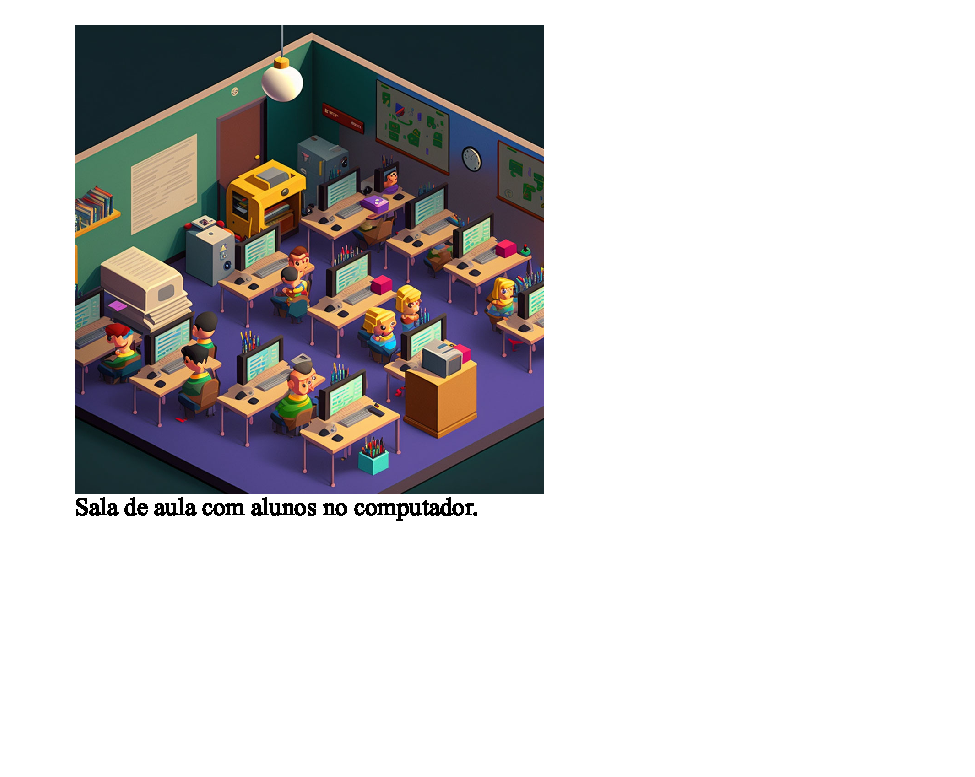
\includegraphics[width=1\textwidth, trim={1cm 4cm 0 0}]{Images/chapter05/imagem03.pdf}}
    \caption{Renderização da imagem com legenda do exemplo \ref{code:fig}.}
    \label{fig:fig}
\end{figure}

Em resumo, as figuras e legendas são uma ferramenta útil para apresentar imagens de forma clara e organizada em uma página web. Ao usar o elemento \var{<figure>} e o elemento \var{<figcaption>}, você pode fornecer informações adicionais sobre a imagem e torná-la mais significativa para o usuário.

\section{Imagens Responsivas}

Para usar imagens de forma responsiva em uma página web, isto é, cujo tamanho se adeque à resolução de tela do dispositivo, você pode usar o recurso de largura e altura do elemento \var{img} (\var{width} e \var{height}). Porém, os valores passados devem estar em percentual. Assim, se a página for aberta em diferentes tamanhos de tela ou se o usuário redimensionar o navegador, a imagem será redimensionada para o percentual relativo à área de visualização disponível.

O redimensionamento proporcional ao tamanho da área de visualização promove a responsividade, porém, essa não é a melhor solução, uma vez que uma mesma imagem será usada para diferentes resoluções de tela. Isso pode desperdiçar banda em dispositivos de tela pequena e gerar imagens ruins em dispositivos de tela grande, pois um único arquivo contendo a imagem com dimensões médias será usado.

O elemento \var{<picture>} é uma maneira eficaz de fornecer imagens responsivas em uma página web. Ele permite que você forneça diferentes versões (arquivos) de uma imagem, cada uma delas otimizada para determinado tamanho de tela. O exemplo \ref{code:picture} mostra como usar o elemento \var{<picture>} para fornecer imagens responsivas.

\begin{htmlcode}{Imagem responsiva com arquivos otimizados.}{code:picture}
<picture>
    <source media="(max-width: 767px)" srcset="imagem-pequena.png">
    <source media="(min-width: 768px)" srcset="imagem-grande.png">
    <img src="imagem-padrao.png" alt="Descrição da imagem" width="100%">
</picture>
\end{htmlcode}

Neste exemplo \ref{code:picture}, o elemento \var{<source>} é usado para especificar diferentes versões da imagem. A primeira versão da imagem é fornecida com o atributo \var{srcset="imagem-pequena.png"} e o atributo \var{media="(max-width:\space767px)"}, o que significa que o arquivo ``imagem-pequena.png'' será usado em telas com largura máxima de 767 pixels. A segunda versão da imagem é fornecida com o atributo \var{srcset="imagem-grande.png"} e o atributo \var{media="(min-width:\space768px)"}, o que significa que o arquivo ``imagem-grande.png'' será usado em telas com largura mínima de 768 pixels.

A imagem padrão é fornecida no próprio atributo \var{src} do elemento \var{<img>}, e será usada em caso de falha ou em navegadores que não suportam o elemento \var{<picture>}. Neste caso, foram fornecidas 3 versões da imagem, mas é possível combinar os valores de \var{min-width} e \var{max-width} para definir imagens compatíveis com telas em uma faixa de tamanho mais específica. Isso abre possibilidades para se fornecer infinitas versões da imagem para os mais diversos tamanhos de tela. Vale ressaltar que o navegador buscará no servidor somente a imagem compatível com a sua resolução de tela.

Em síntese, o elemento \var{<picture>} permite que você forneça imagens responsivas, oferecendo diferentes versões da imagem para diferentes tamanhos de tela. Ao usar o elemento \var{<source>} e os atributos \var{media} e \var{srcset}, você pode especificar quando cada versão da imagem deve ser usada, garantindo que a imagem correta seja carregada e exibida para cada tamanho de tela.

\section{Mapas de Imagens}

Os mapas de imagem são uma técnica popular para criar links em regiões dentro de imagens em HTML. Eles permitem que diferentes áreas da imagem sejam associadas a links diferentes, criando uma maneira interativa e atraente de navegar em um site. Um mapa de imagem pode ser utilizado para diversos fins, desde criar links para diferentes áreas de um produto em uma loja virtual até adicionar interatividade em uma página de informações turísticas a partir de um mapa geográfico do local.

Em HTML, um mapa de imagem é criado utilizando o elemento \var{<map>} juntamente com elementos do tipo \var{<area>}. As áreas da imagem são definidas utilizando o atributo \var{coords}, que define as coordenadas dos pontos que formam a área clicável da imagem, e o atributo \var{shape}, que define a forma da área da imagem (por exemplo, retangular, circular ou poligonal).

Ao clicar em uma área definida no mapa de imagem, o usuário é redirecionado para destino específico, funcionando como um link. Os mapas de imagem também podem ser utilizados para criar efeitos de destaque, como a exibição de informações adicionais sobre uma área específica da imagem quando o usuário passa o mouse sobre ela.

Nesta seção, exploraremos como criar e usar mapas de imagem em HTML. Vamos começar entendendo os conceitos básicos de como as áreas são definidas e como criar um mapa de imagem simples. Em seguida, discutiremos como adicionar diferentes formas de áreas, como polígonos, retângulos e círculos, e como adicionar links.

\subsection{Um Mapa de Imagem Simples}

Para criar um mapa de imagem simples em HTML, vamos ter que seguir alguns passos. O primeiro deles é identificar quais são as regiões da imagem que você quer tornar clicável. Para verificarmos isso, vamos considerar a imagem da figura \ref{fig:formas}.

\begin{figure}[ht!]
    \frame{
    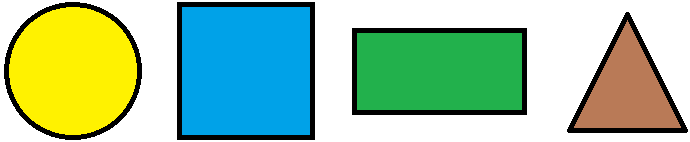
\includegraphics[width=1\textwidth]{Images/chapter05/formas.png}}
    \caption{Imagem simples com 4 formas geométricas, com dimensões 690x142 pixels. \\(Disponível em \url{https://imgbox.com/KAP9OMBi})}
    \label{fig:formas}
\end{figure}

Imagine que precisemos tornar cada forma geométrica clicável, obedecendo precisamente seus limites. Vamos começar adicionando a imagem à página web utilizando o elemento \var{<img>}. Certifique-se de apontar o atributo \var{src} para o caminho correto da imagem e de definir o atributo \var{alt} para fornecer uma descrição alternativa da imagem, que é importante para fins de acessibilidade. O código inicial é mostrado no exemplo \ref{code:mapa1}.

\begin{htmlcode}{Código inicial do mapeamento de imagem.}{code:mapa1}
<img src="formas.png" alt="Formas geométricas">
\end{htmlcode}

Agora que temos a imagem, temos que criar um elemento \var{<map>} para definirmos o mapeamento. É importante também fornecermos um nome para este elemento \var{<map>} através de seu atributo \var{name}. O exemplo \ref{code:mapa2} mostra o código até este momento.

\begin{htmlcode}{Imagem e mapa de imagem.}{code:mapa2}
<img src="formas.png" alt="Formas geométricas">
<map name="mapaFormas">
</map>
\end{htmlcode}

Agora, dentro do elemento \var{<map>}, temos que adicionar um elemento \var{<area>} para cada região que queremos mapear, sendo que cada elemento \var{<area>} deve ter um atributo \var{shape}, que define a forma da área, e um atributo \var{coords}, que define as coordenadas da área em relação à imagem. Vamos começar mapeando o círculo amarelo. Primeiramente, temos que descobrir as coordenadas do centro do círculo. Vale ressaltar que a coordenada (0,0) está localizada no canto superior esquerdo da imagem, portanto, quanto mais à direita, mais próximo de 690 fica o valor da coordenada X, e quanto mais para baixo, mais próximo de 142 fica o valor da coordenada Y.

Para descobrir as coordenadas do centro desse círculo, eu abri essa imagem no \textit{Paint}, editor de imagens básico do \textit{Windows}, posicionei o cursor do mouse no centro do círculo, e olhei na barra de status na parte inferior as coordenadas do cursor do mouse. O valor mostrado, neste caso, foi de (73,69), portanto, essas são as coordenadas do centro do círculo amarelo. Agora, eu preciso saber o valor do raio do círculo. Para isso, eu posiciono o cursor do mouse na extremidade direita do círculo, vejo o valor da coordenada X, e subtraio da coordenada X do centro. Neste caso, a coordenada X da extremidade vale 142, portanto, o raio vale 69. Agora temos que criar um elemento \var{<area>} do tipo ``círculo'' e passar esses valores. O exemplo \ref{code:mapa3} mostra como está ficando o código até aqui.

\begin{htmlcode}{Imagem e mapa de imagem com uma área clicável.}{code:mapa3}
<img src="formas.png" alt="Formas geométricas">
<map name="mapaFormas">
    <area shape="circle" coords="73,69,69" href="circulo.html" alt="Círculo amarelo">
</map>
\end{htmlcode}

Na linha 3 do exemplo \ref{code:mapa3}, temos o elemento \var{<area>}. Veja o atributo \var{shape="circle"}, indicando que essa área é um círculo. Isso é importante para que o elemento interprete corretamente as coordenadas que estão no atributo \var{coords}. Sempre que \var{shape="circle"}, as coordenadas passadas devem corresponder ao centro do círculo e ao raio do círculo. Por isso o valor do atributo \var{coords} é igual a \var{73,69,69}, pois os dois primeiros valores correspondem às coordenadas X,Y do centro do círculo e o terceiro valor corresponde ao raio. O atributo \var{href} contém o endereço do link correspondente à região, ou seja, para onde o usuário será redirecionado quando clicar no círculo. Por fim, o atributo \var{alt} promove a acessibilidade através de uma descrição da imagem.

Vamos prosseguir criando uma região clicável para o quadrado azul. Neste caso, temos que usar o atributo \var{shape="rect"} e passar como coordenadas os valores X,Y do canto superior esquerdo e os valores X,Y do canto inferior direito. Você pode obter esses valores usando a mesma técnica utilizada para o círculo amarelo, com o \textit{Paint} ou outro editor de imagem. Eu obtive as coordenadas (177,2) para o canto superior esquerdo e (314,139) para o canto inferior direito do quadrado azul. Aproveitando que a próxima forma é um retângulo verde e, consequentemente, usa o mesmo tipo de \var{shape} do quadrado, eu analisei as coordenadas dos cantos do retângulo verde e cheguei as valores (352,28) e (526,114). Portanto, eu vou agora complementar o código com novas áreas para essas formas. O exemplo \ref{code:mapa4} mostra como ficou o código até aqui.

\begin{htmlcode}{Imagem e mapa de imagem com uma área clicável.}{code:mapa3}
<img src="formas.png" alt="Formas geométricas">
<map name="mapaFormas">
    <area shape="circle" coords="73,69,69" href="circulo.html" alt="Círculo amarelo">
    <area shape="rect" coords="177,2,314,139" href="quadrado.html" alt="Quadrado azul">
    <area shape="rect" coords="352,28,526,114" href="retangulo.html" alt="Retângulo verde">
</map>
\end{htmlcode}

Se você tentar clicar nas regiões com o código como está, verá que ainda não funciona. Isso acontece porque, apesar de nosso mapa já definir 3 regiões, nós ainda não informamos para a imagem que ela deve usar o mapa em questão. Para fazer isso, temos que ir até o elemento \var{<img>} e passar o atributo \var{usemap="\#mapaFormas"}. Faça isso e teste. Eu vou deixar para mostrar esse trecho junto com o próximo código, portanto, vamos a ele.

Agora vamos adicionar a região do triângulo vermelho. Acontece que essa região não é circular e nem retangular, portanto, não podemos usar os tipos \var{circle} e \var{rect} no atributo \var{shape}. Para polígonos quaisquer, devemos usar o tipo \var{poly} passando as coordenadas de cada vértice do polígono em ordem. Eu vou adotar o sentido horário, portanto, vou ver qual é a posição do vértice superior do triângulo, do direito e do esquerdo, nesta ordem. Os valores que obtive foram (627,12), (688,132) e (566,132), respectivamente. O exemplo \ref{code:mapa5} mostra a versão final do mapa incluindo as 4 áreas e o atributo \var{usemap} no elemento \var{img}.

\begin{htmlcode}{Versão final do mapeamento da imagem de formas geométricas.}{code:mapa5}
<img src="formas.png" alt="Formas geométricas" usemap="#mapaFormas">
<map name="mapaFormas">
    <area shape="circle" coords="73,69,69" href="circulo.html" alt="Círculo amarelo">
    <area shape="rect" coords="177,2,314,139" href="quadrado.html" alt="Quadrado azul">
    <area shape="rect" coords="352,28,526,114" href="retangulo.html" alt="Retângulo verde">
    <area shape="poly" coords="627,12,688,132,566,132" href="triangulo.html" alt="Triângulo vermelho">
</map>
\end{htmlcode}

Obviamente, se você tiver que mapear polígonos complexos, a tarefa não será muito fácil. Imagine, por exemplo, se você tiver que mapear cada Estado em um mapa do Brasil. Serão muitos vértices! Bem, neste caso, eu aconselho o uso de alguma ferramenta auxiliar. O site \url{https://www.image-map.net} permite que você faça o \textit{upload} de uma imagem e crie o mapeamento de regiões de forma bem mais conveniente do que a que mostrei aqui. Sugiro que explore essa ferramenta caso tenha que fazer mapeamentos mais complexos.

\section{Imagens Como Links}

Em HTML, você pode usar imagens como links envolvendo um elemento \var{<img>} correspondente à imagem com um elemento \var{<a>} correspondente ao link. Quando o usuário clicar na imagem, ele será redirecionado para a página vinculada ao link. O exemplo \ref{code:img_link} mostra o código de uma imagem sendo usada como link.

\begin{htmlcode}{Imagem como link.}{code:img_link}
<a href="contato.html">
  <img src="telefone.png" alt="Link para a página de contato">
</a>
\end{htmlcode}

\section{Exercícios Propostos}

Essa série de exercícios envolve os conceitos abordados neste capítulo e também \textbf{pode demandar alguma pesquisa}. Reserve um tempo e um local adequados para fazer os exercícios sem distrações. Assim você absorverá muito mais o conteúdo estudado.

\begin{exercise}
Crie uma imagem com o atributo \var{src} apontando para o arquivo ``imagem.jpg'' e com um texto alternativo ``Imagem de um gato''.
\end{exercise}

\begin{exercise}
Crie uma imagem para o arquivo local ``cachorro.jpg'' com uma largura de 400 pixels e uma altura de 300 pixels.
\end{exercise}

\begin{exercise}
Crie uma imagem com largura de 300 pixels contendo uma foto do planeta Saturno, sendo que essa foto deve estar em um endereço externo obtido via buscador.
\end{exercise}

\begin{exercise}
Crie uma imagem para o arquivo ``logo.png'' e com texto alternativo ``Logotipo da empresa'', que seja um link para a página externa ``https://exemplo.com''.
\end{exercise}

\begin{exercise}
Crie um elemento \var{<picture>} com duas resoluções diferentes de imagens, uma para telas de até 720px de altura e outra para telas com altura maior que 720px. Use nomes de arquivos fictícios.
\end{exercise}

\begin{exercise}
Crie um elemento \var{<picture>} com imagens diferentes para telas em formato ``retrato'' e telas em formato ``paisagem''. Use nomes de arquivos fictícios. (pesquise como configurar o atributo \var{media} para essa situação).
\end{exercise}

\begin{exercise}
Crie um mapeamento para a imagem disponível em \url{https://tinyurl.com/3j558uax}, de forma que cada logotipo aponte para o site da respectiva empresa. Mostre a imagem com 800px de largura.
\end{exercise}

\begin{exercise}
Crie um mapeamento para a imagem disponível em \url{https://tinyurl.com/3bu9ekz3}, de forma que cada região do Brasil aponte para um arquivo HTML com seu nome (norte.html, nordeste.html etc.). Mostre a imagem com 800px de largura.
\end{exercise}

\section{Considerações Sobre o Capítulo}

Este capítulo apresentou como exibir imagens usando HTML. Vimos como mostrar imagens simples, imagens responsivas que se ajustam ao tamanho a tela, carregamento otimizado de imagens responsivas e mapeamento de imagens. No capítulo seguinte veremos como apresentar imagens em um documento HTML.